\section{Systemübersicht}

\subsection{Lösungsstrategie}
Um die verteilte Dokumentenbearbeitung zu ermöglichen, verwenden wir eine Variante von Eventsourcing.
Dabei sollen die alle Änderungen am Dokument als einzelne Commands modelliert werden.
Commands werden von Clients generiert, lokal angewendet und anschliessend an den Server gesendet.
Dieser führt den Zustand des Dokuments und wendet Änderungen darauf an.
Allfällige Konflikte werden dabei auf dem Server gelöst.
Nach der Verarbeitung eines Commands veröffentlicht der Server alle angewendeten Commands sowie Commands zur Konfliktlösung.
Diese Commands werden wiederum von den Clients angewendet, um einen konsistenten Zustand des Dokuments herzustellen.
Commands werden in einer Datenbank persistiert.

Dieser Ansatz erlaubt es Änderungen nachzuvollziehen und bei Bedarf einen früheren Zustand des Dokuments wiederherzustellen.
Das Führen des Zustands auf dem Server erlaubt es, eine ''Source Of Truth'' zu haben, die den gültigen Zustand des Dokuments diktiert.
Das Anwenden von Commands in den Clients erlaubt es auch dort einzelne Änderungen nachzuvollziehen und darzustellen.

\subsection{Technologien und Systemaufbau}

Das Versenden von Commands findet über zwei getrennte Kanäle statt.
Für Versenden von Commands vom Backend an Clients verwenden wir HTTP-Event Streams (Server Sent Events).
Als konkrete Implementation dieser Technologie setzen wir Spring-WebFlux ein.
Die weitere Technologieauswahl orientiert sich an diesem Grundsatz Entscheid.
Für das Versenden von Commands von Clients an das Backend werden HTTP-POST-Requests verwendet.
Diese Trennung erlaubt es, das Schreiben und Lesen von Änderungen zu trennen.

\subsubsection{Backend Server}

Für das Backend wird eine Spring Boot Applikation mit Spring Webflux erstellt.
Dieser Ansatz ermöglicht es, eine reaktive Serverapplikation zu erstellen, welche mit minimalem Boilerplate Code auskommt.

Das Spring Boot Ökosystem benötigt eine zugrundeliegende JVM\@.
Sprachen die auf der JVM aufbauen, haben den Vorteil, dass sie System Interoperabel sind.
Anstatt Java setzen wir jedoch auf Kotlin als Backend Sprache.
Bis jetzt hat kein Mitglied des Projektteams nennenswerte Erfahrung mit Kotlin oder reaktiver Programmierung.
Wir möchten diese Gelegenheit nutzen, die Sprache in einem Projekt näher kennenzulernen.
Wir erhoffen uns vom Einsatz von Kotlin folgende Vorteile:

\begin{itemize}
    \item Robuste Implementierung dank Null Safety
    \item Weniger Boilerplate und damit übersichtlichere Implementeirung
    \item Effiziente und Übersichtliche Anwendung von Streams
\end{itemize}

\subsubsection{Frontend Clients}

Für die Client-Applikation wird das Framework React eingesetzt.
React bietet mit seinem Komponenten-Model eine einfache Abstraktionsmöglichkeit um die Anwendung sauber zu Kapseln.
Die Funktionalen React Komponenten scheinen leichtgewichtiger im Vergleich zu den HTML-Template-Ansätzen von Angular oder VueJS\@.
Das Projektteam hat bis jetzt noch keine grösseren Projekte mit React umgesetzt.
Unser Ziel ist es in diesem Projekt die React Kenntnisse in einem Projekt zu vertiefen und die Client-Software möglichst pur funktional zu halten.

Änderungen am Dokument werden auch im Frontend immer als Commands modelliert.
Für die Verarbeitung dieser Commands und das Verwalten des Zustands der Client Applikation wird redux verwendet.

\begin{figure}[h]
    \centering
    \begin{minipage}[b]{\textwidth}
        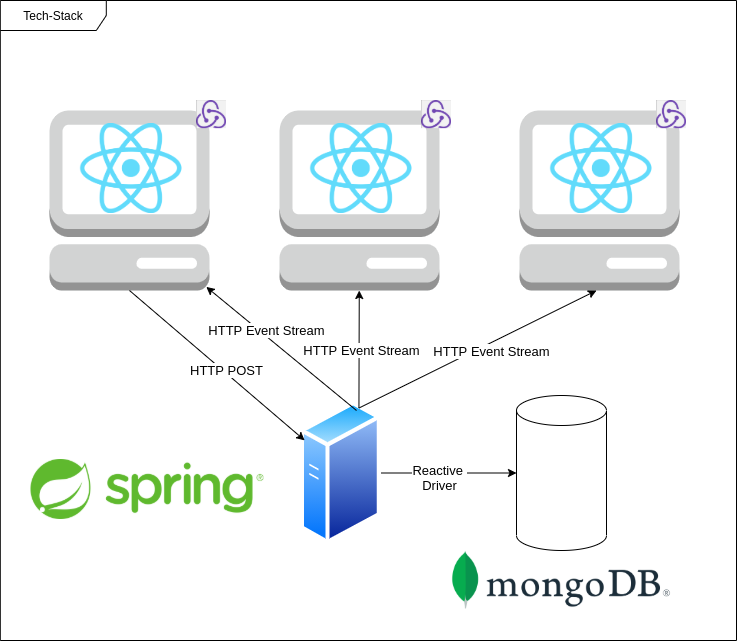
\includegraphics[width=\textwidth]{images/TechStack2.drawio}
        \caption{Technologie Stack}
    \end{minipage}\label{fig:figstack}
\end{figure}

\subsubsection{Datenbank System}
Um die kollaborativ erstellten Dokumente zu persistieren und zu verwalten setzen wir auf eine No-SQL Lösung.
Das notwendige Datenmodel lässt sich elegant als \emph{Document} abbilden.
Durch den Einsatz einer No-SQL Lösung kann die Representation der Dokumente über alle Layer der Applikation gleichbleibend beibehalten werden\@.
Konkret wird im Projekt MongoDB als Datenbanksystem verwendet.
Wir haben uns für diese Variante aufgrund der bestehenden reaktiven Integration in das Springframework entschieden.

\clearpage

\subsection{Applikationsprotokoll}
In der Folge wird auf die verschiedenen Kanäle und das Applikationsprotokoll eingegangen.

\subsubsection{EventSource}
Für die stetige Verbindung der Clients zum Server abonnieren die Clients eine EventSource.
Die EventSource ist eine langlebige HTTP Verbindung.
Über diese Verbindung hören alle Clients auf Änderungen, die von anderen Clients gemacht werden.
Dieser Kanal sendet alle Commands einzeln an die Clients.
Im Fehlerfall wird die Verbindung geschlossen.
Clients können die Verbindung darauf erneut, öffnen um den aktuellen Zustand des Dokuments zu erhalten.
Damit wird ein konsistenter Zustand erstellt.
Die EventSource wird auch verwendet, um eine Aussage über die verbundenen Clients machen zu können.

\subsubsection{HTTP}
Die Clients wenden im Frontend alle Commands auf sich selber an und senden danach das Command an den Server.
Dafür gibt es einen HTTP POST Endpunkt, der alle Commands entgegennimmt.
Intern wird anhand des "type" in der Payload entschieden, wie mit dem Command umgegangen wird.
Die genaue Übersicht der Endpunkte ist im Kapitel "API" zu finden.
Eine Beschreibung der implementierten Typen ist im Kapitel 5 beschrieben.

\subsubsection{Applikationsprotokoll}

Frontend und Backend tauschen Commands im JSON-Format aus.
Dabei haben die ausgetauschten Objekte folgenden Aufbau:

\begin{itemize}
    \item type: Der Command Type (Bsp. ADD\_PARAGRAPH)
    \item payload: Ein JSON Objekt welches die Payload für den konkreten type enthält
    \item sender: Eine eindeutige ID des Senders
    \item (opt.) correlationId: ID der payload eines anderen Commands
\end{itemize}

\subsection{Benutzerverwaltung}
Es ist keine persistente Benutzerverwaltung mit Registrationsprozess implementiert.
Nach erstmaligem Anmelden in der Applikation mit einem globalen Benutzer, wird ein zufälliger Author erstellt.
Die Daten des Authors werden im Local Storage des Browsers gespeichert, sodass bei erneutem Öffnen der Applikation der gleiche Author wiederverwendet wird.
